% Figure from MATH 591 notes, section 3. Compile with the notes preamble.
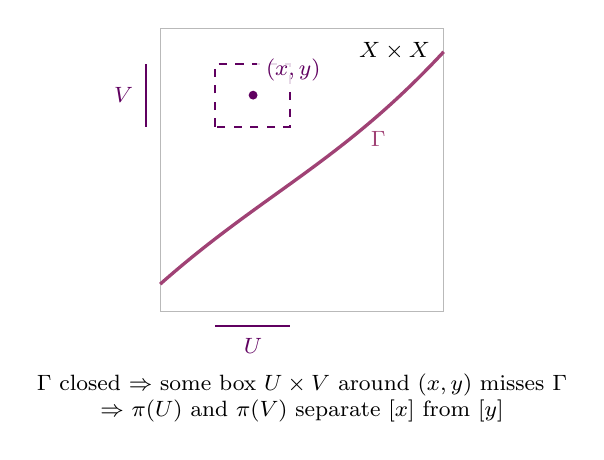
\begin{tikzpicture}[scale=1.0]
\draw[gray!55] (0,0) rectangle (3.6,3.6);
\node[font=\footnotesize,anchor=north east] at (3.55,3.55) {$X\times X$};
\draw[magenta!60!black,very thick] (0,0.35) .. controls (1.3,1.5) and (2.3,1.9) .. (3.6,3.3);
\node[magenta!60!black,font=\footnotesize,anchor=west] at (2.55,2.2) {$\Gamma$};
\draw[dashed,violet!75!black,thick] (0.7,2.35) rectangle (1.65,3.15);
\fill[violet!75!black] (1.18,2.75) circle (1.6pt);
\node[fill=white, fill opacity=0.85, text opacity=1, text=violet!75!black,font=\footnotesize,anchor=south west] at (1.22,2.8) {$(x,y)$};
\draw[violet!75!black,thick] (0.7,-0.18) -- (1.65,-0.18);
\node[violet!75!black,font=\footnotesize,below] at (1.18,-0.22) {$U$};
\draw[violet!75!black,thick] (-0.18,2.35) -- (-0.18,3.15);
\node[violet!75!black,font=\footnotesize,left] at (-0.22,2.75) {$V$};
\node[font=\footnotesize,align=center] at (1.8,-1.1) {$\Gamma$ closed $\Rightarrow$ some box $U\times V$ around $(x,y)$ misses $\Gamma$\\ $\Rightarrow$ $\pi(U)$ and $\pi(V)$ separate $[x]$ from $[y]$};
\end{tikzpicture}
